\chapter{基于知识的情感分析模型}\thispagestyle{fancy}
本章首先介绍了基于知识的情感分析模型所使用到的Stanford语法树,然后介绍了知识模型的主要思想和基本实现步骤。关于知识模型的性能分析详见\nameref{sec:modeleval}。
\section{知识模型简介}
基于情感词典的情感分类方法是基于知识的情感分类方法中的主流方法,本文所实现的知识模型也主要利用情感词典完成情感极性和情感强度的判定。但单纯通过情感词典判定单词或者短语的情感强度常常忽略说话者的隐含信息,如"她聪明但很令人讨厌",其中聪明是正向形容词,"令人讨厌"是负向形容词,正向词与负向词的比例为1:1,恰好平衡,可能为矛盾情感,而实际上,因为"但是"起转折作用,"很"起强调作用且二者都与"令人讨厌"有关,该句的情感极性应该为负向。为了利用修饰关系或者语法特征,研究者们往往需要编写复杂的规则如\cite{Choi2008},这容易导致程序过于复杂,不易维护和拓展。基于语法树的方法则能通过利用语法树的层级关系判断句式和词语之间的依赖关系和作用范围,更加简便地处理情感传播,极性冲突和极性转换等问题\cite{Moilanen2007}。


本文实现的知识模型主要使用Stanford 语法树和\nameref{sec:emotionset}所介绍的情感词典。该知识模型通过top-down方式,由语法树的根节点向叶节点递归,由词典或子节点推测每个节点的程度强度或情感强度。由于语法树的使用,知识模型往往可以避免引入冗长的规则,仅使用简单的规则处理复杂句式。例如,对于双重否定句"这家酒店不是不好。","好"的情感强度为+1.0,而"不"起否定作用,程度强度为-1.0,这会导致节点"不好"的情感为-1.0,而"不是"与"不好"是"不是不好"的子节点,而"不是"的程度强度也为-1.0,最后,"不是不好"的结果为+1.0,这与双重否定句所代表的实际语义相符。该模型不需要训练,适合处理情感较为强烈,使用情感词较多,语法较为规范的语句。


本文主要使用两个词典,一个为情感词典emotion,另一个为程度词典degree。emotion中的词条为情感词及对应强度,degree中的词条为程度词和对应强度。在词典中,强度可能为+2.0,+1.5,+1.0,+0.5,-0.5,-1.0,-1.5,-2.0。对于情感词来说,如果某情感词为正向词,则其对应强度为正数,反之,如果某情感词为负向,则其对应强度为负数。如"高兴"强度为1.0,"沉痛"强度为-2.0。对于强度词来说,如果某个词起强调作用,则强度为正数,起转折作用,则其强度为负数。例如"很"的强度为+2.0,"不"的强度为-1.0。


\section{Stanford 语法树}
Stanford Parser是由斯坦福自然语言处理小组实现的语法分析工具,也是Stanford CoreNLP的其中一个组件。它主要基于概率上下文无关文法(Probabilistic Context Free Grammar,PCFG,又称随机上下文无关文法,Stochastic Context Free Grammar,SCFG),能进行句法分析和语义依存分析(Semantic Dependency Parsing, SDP),生成语法树和依赖关系,是目前比较主流的一款语法分析工具。\par
本文选择Stanford Parser作为句法分析器,因此在此简单介绍Stanford Parser的中心算法思想。\par

定义:一个概率上下文无关文法是一个五元组($N,\Sigma ,S,R,P$),其中$N$为非终结符集,$\Sigma$为终结符集,$S\in N$为开始符集,$R$为产生式集,对于任意产生式$r \in R$,其概率为$P(r)$。规则表示形式为:$A\rightarrow\alpha$,其中$A$为非终结符,$p$为$A$推导出$\alpha$的概率,即$p = P(A\rightarrow\alpha)$,该概率分布必须满足如下条件:$\sum{P(A\rightarrow\alpha)}=1$
\cite{Cha93}\par
对应于语法树,$N$相当于非叶节点,$\Sigma$为叶节点,$S$唯一且$S$为根节点,$R$为可行的路径,$P$为使用某条路径转移的概率。\par
在实践中,$P(A\rightarrow\alpha)$一般设为训练集语料中$A\rightarrow\alpha$的最大似然估计,也即$P(A\rightarrow\alpha) = \frac{Count(A\rightarrow\alpha)}{Count(A)}$,其中$Count(A\rightarrow\alpha)$为已标注语料中出现该规则的次数,$Count(A)$为语料中出现该语法单元的次数。给定语法树后,就能计算出已标注词性的文本符合语法树的概率,而寻找对应的语法树可以转化为动态规划问题求解。\par
明显,PCFG是CFG(上下文无关算法)的拓展,但上下文算法不含概率,无法解决语言的二义性问题,因此PCFG要比CFG更适合于自然语言处理。\par
但由于PCFG等价地对待词组中的所有词,导致相同结构的PCFG对词汇信息和结构偏向不明显。词汇化的PCFG文法为每个语法树的每个节点添加首要词(HEAD),从而克服了PCFG文法的弱点,取得了巨大的成功\cite{Klein2003b}。\par
本文使用Factor模型,在Stanford Parser Factor模型中词汇化的PCFG方法用于同时表示语法结构与依赖关系,如图\ref{fig:parser1}c。Klien等\cite{Klein2003a} 人认为,设$L$为词汇化的PCFG树,则$L$可以被一棵语法PCFG树$T$(如图\ref{fig:parser1}a)和一棵结构相符合的依赖关系树$D$(如图\ref{fig:parser1}b)确定。于是,基于文本构建$L$的问题就被转化为基于文本构建一对$T$,$D$,使$P'(T,D)$最大,这里$P'(T,D)$代表文本同时符合$T$,$D$的概率。Klein等人进一步假设$T$与$D$相对独立,也即$P'(T,D) = P'(T)P'(D)$,并分别使用动态规划构建概率最大的$T$,$D$,之后使用A*启发式算法搜索T和D的近似结合方式,该算法取得了不错的成果。\par
Stanford Parser还对分析器做了一系列优化\cite{LevyM03} \cite{Marneffe06} \cite{Zhang2011} \cite{ChenM14} \cite{SocherBMN13} \cite{Nivre16} \cite{SchusterM16},在此不做赘述。
\begin{figure}
\begin{center}
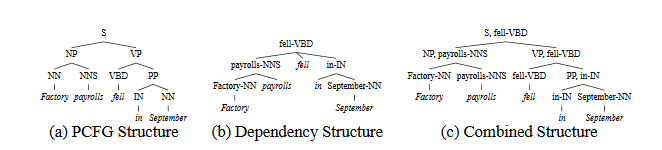
\includegraphics[width=\textwidth]{graphic/parser1.PNG}
\caption{三种分析结构 \label{fig:parser1}}
\end{center}
\end{figure}
\section{基本流程}
算法基本流程如图\ref{fig:plain1}\par
\begin{figure}
\begin{center}
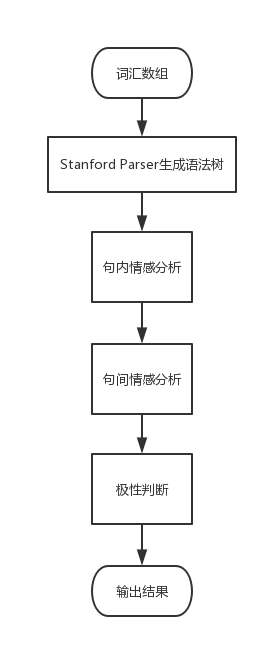
\includegraphics [width=0.6\textwidth, height=10cm]{graphic/plainmodel1.png}
\caption{知识模型基本流程图 \label{fig:plain1}}
\end{center}
\end{figure}
伪代码如下:\par
\lstset{language=python}
\begin{lstlisting}
def analyze(words, lang):
  if lang == 'zh':
    trees = parser_zh.parse(words)
  else:
    trees = parser_en.parse(words)
  ans = 0
  for tree in trees:
    dfs(tree.root,tree)
    ans += tree.root.sentiment
  
  if ans == 0:
    if tree has child whose sentiment != 0:
      return contradict
    else:
      return neural
  else if ans > 0:
    return positive
  else:
    return negative

def dfs(node, tree):
  node.phrase = ''
  if not isleaf(node):
    for child in node.daughterTrees:
      dfs(child, tree)
  if isleaf(node):
    node.phrase = node.label
  else:
      for child in node.daughterTrees:
        if lang == 'zh':
          node.phrase = node.phrase + child.phrase
        else:
          if isW(child) or child.label == "n't":
            node.phrase = node.phrase + child.phrase
          else:
            node.phrase = node.phrase + ' ' + child.phrase
  found, node.sentiment = lookup_in_emotion(node.phrase)
  if not found:
    found, node.sentiment = lookup_in_degree(node.phrase)
  if not found:
    if not isleaf(node):
      d = 0
      e = 0
      for child in daughterTrees:
        if child.label == 'RB'
          or child.label == 'VE'
          or child.label == 'AD':
          d += child.sentiment
        else:
          e += child.sentiment
      if d == 0:
        node.sentiment = e
      elif e == 0:
        node.sentiment = d
      else:
        node.sentiment = d * e
\end{lstlisting}


算法首先将分词后的词汇输入到Stanford Parser中,每个短句将生成一棵独立的语法树。


接着算法对每个短句所生成的语法树采用top-down递归遍历。


在递归的过程中,算法会首先在词典中查找子树所对应的短语,如果找到了对应的短语,则将短语所代表的情感强度或者程度强度设为该子树的强度,否则,分别统计子树的子节点的情感强度和程度强度,取其乘积作为该子树的强度。


最后,算法将多棵语法树根节点的情感强度相加,得到整体情感强度。如果整体情感强度大于0,则最终情感极性为正向,如果整体情感小于0,则最终情感极性为负向,如果整体情感强度等于0且子树情感强度都为0,则为中性,如果整体情感强度等于0,但存在子树情感强度不为0,则为矛盾情感。


如图,对于“This is the right size for any use!  Uses little space and looks extremely good on the counter.”,Stanford Parser将会生成如图\ref{fig:plainf2}的结果。

\begin{figure}
\begin{center}
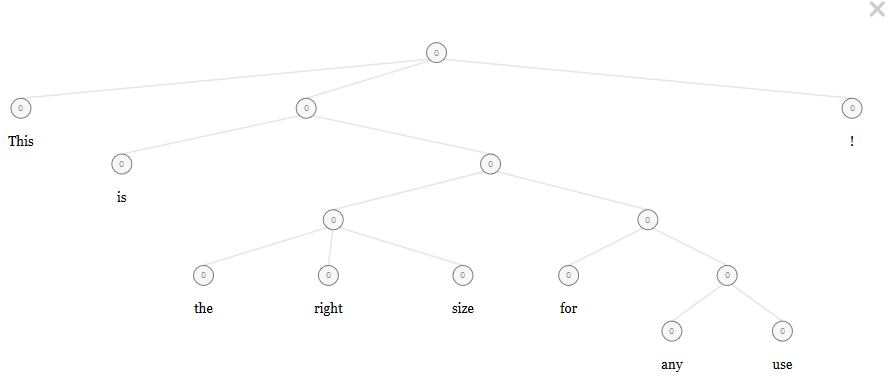
\includegraphics[width=\textwidth]{graphic/plainmodel2.png}
\caption{语法树可视化 \label{fig:plainf2}}
\end{center}
\end{figure}


算法分别从左右两棵树根节点开始分析,逐步到达叶节点,以右边的树为例,该树对应"Uses little space and looks extremely good on the counter."。\par
\begin{enumerate}
\item 在情感词典中,"little"的情感强度为-1.0,因此"little space","Use little space"的情感强度都被标注为-1.0。
\item "extremely"在程度词典中被标注为+2.0,"good"在情感词典中被标注为+1.0,因此"extremely good", "looks extremely good on the counter."被标注为+2.0
\item 综上,"Uses little space and looks extremely good on the counter."被标注为+1.0
\item 右边的树也遵循此流程,极性为+1.0,将子句合并考虑,得到该语句整体情感强度为+2.0。
\item 由于算法将大于0的结果定为正向,所以该评论文本的整体情感为正向。
\end{enumerate}\par
最终,算法可视化结果如图\ref{fig:plainf3}。


\begin{figure}
\begin{center}
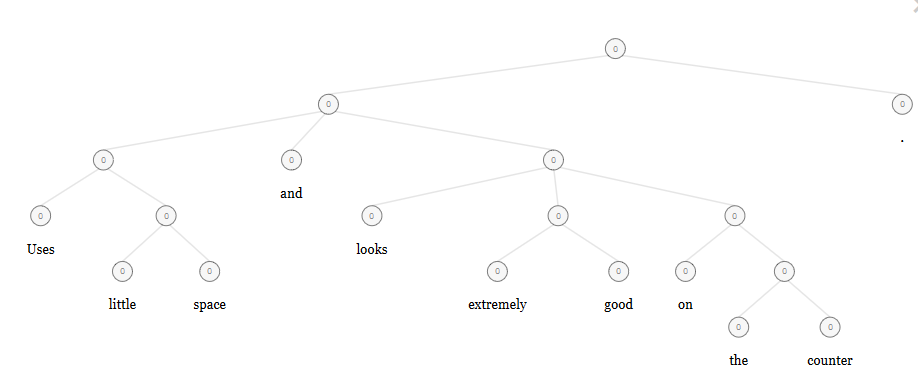
\includegraphics[width=\textwidth]{graphic/plainmodel3.png}
\caption{知识模型算法结果可视化 \label{fig:plainf3}}
\end{center}
\end{figure}
